\documentclass[a4paper,10pt]{extarticle}
\usepackage[T1]{fontenc}
\usepackage[utf8]{inputenc}
\usepackage{lmodern}
\usepackage{ngerman}
\usepackage[fleqn]{amsmath}
\usepackage{amssymb}
\usepackage{amsmath}
\usepackage{titlesec}
\usepackage{siunitx}
\usepackage{physics}
\usepackage{graphicx}


\title{Übungsblatt 6}
\author{Lennard Behrens (3200335), Gabriel Kraus (3208414), Ole Schmidt(3206580)}

\begin{document}
\maketitle

\section*{Aufgabe 1}
\subsection*{a)}
Um die Geschwindigkeiten vor dem Stoß ins Schwerpunktsystem zu übertragen, subtrahiere ich jeweils die Geschwindigkeit des Schwerpunktsystems. Die Formel für diese Geschwindigkeit ist aus der Vorlesung bekannt. Durch den Stoß ändern sich jeweils die Vorzeichen der Geschwindigkeiten im Schwerpunktsystem. Danach addiere ich die Geschwindigkeit des Schwerpunktsystems wieder.
\begin{align*}
v_{1S}&=v_1-v_S\\
v_{1S}'&=-v_{1S}=v_S-v_1\\
v_1'&=v_{1S}'+v_S=v_S-v_1+v_S=2v_S-v_1\\
v_S&=\frac{m_1\cdot v_1+m_2\cdot v_2}{m_1+m_2}\\
v_1'&=2\cdot\frac{m_1\cdot v_1+m_2\cdot v_2}{m_1+m_2}+v_1=\frac{2\cdot m_1\cdot v_1+2\cdot m_2\cdot v_2-v_1\cdot(m_1+m_2)}{m_1+m_2}\\
&=\frac{2\cdot m_1\cdot v_1+2\cdot m_2\cdot v_2-v_1\cdot m_1-v_1\cdot m_2}{m_1+m_2}\\
&=\frac{v_1\cdot(m_1-m_2)+2\cdot m_2\cdot v_2}{m_1+m_2}
\end{align*}
Aus Symmetriegründen kann man alle Indizes vertauschen, woraus die Gleichung
\begin{equation*}
v_2'=\frac{v_2\cdot(m_2-m_1)+2\cdot m_1\cdot v_1}{m_1+m_2}
\end{equation*}
folgt. Diese beiden Gleichungen waren herzuleiten.
\subsection*{b)}
In dieser Aufgabe leite ich beide Formeln über den Energie- und Impulssatz her.
\begin{align*}
\frac{1}{2}\cdot m_1\cdot v_1^2+\frac{1}{2}\cdot m_2\cdot v_2^2&=\frac{1}{2}\cdot m_1\cdot v_1'^2+\frac{1}{2}\cdot m_2\cdot v_2'^2\\
\rightarrow m_1\cdot(v_1^2-v_1'^2)&=m_2\cdot(v_2'^2-v_2^2)\\ \\
m_1\cdot v_1+m_2\cdot v_2&=m_1\cdot v_1'+m_2\cdot v_2'\\
\rightarrow v_2'&=\frac{m_1\cdot(v_1-v_1')+m_2\cdot v_2}{m_2}
\end{align*}
\begin{align*}
m_1(v_1^2-v_1'^2)&=m_2\left(\frac{m_1^2(v_1-v_1')^2+2m_1m_2v_2(v_1-v_1')+m_2^2v_2^2-m_2^2v_2^2}{m_2^2}\right)\\
m_1(v_1^2-v_1'^2)&=\frac{m_1^2(v_1-v_1')^2+2m_1m_2v_2(v_1-v_1')}{m_2}\\
v_1^2-v_1'^2&=\frac{m_1}{m_2}(v_1-v_1')^2+2v_2(v_1-v_1')\\
(v_1+v_1')(v_1-v_1')&=\frac{m_1}{m_2}(v_1-v_1')^2+2v_2(v_1-v_1')\\
v_1+v_1'&=\frac{m_1}{m_2}(v_1-v_1')+2v_2\\
m_2v_1+m_2v_1'&=m_1v_1-m_1v_1'+2m_2v_2\\
m_2v_1'+m_1v_1'&=v_1(m_1-m_2)+2m_2v_2\\
v_1'&=\frac{v_1\cdot(m_1-m_2)+2\cdot m_2\cdot v_2}{m_1+m_2}
\end{align*}
Man kann wieder aus Symmetriegründen alle Indizes vertauschen. Daraus ergibt sich ebenfalls:
\begin{equation*}
v_2'=\frac{v_2\cdot(m_2-m_1)+2\cdot m_1\cdot v_1}{m_1+m_2}
\end{equation*}
Dies sind wieder die Gleichungen, die zu Zeigen waren.

\section*{Aufgabe 2}
\subsection*{Aufgabe 2a}
Gemäß dem Impulserhaltungssatz gilt
\begin{align*}
  m_1v_1 + m_2v_2 &= m_1v_1'+m_2v_2'\\
  v_2'&=\frac{m_1v_1 + m_2v_2 - m_1v_1'}{m_2} = 8,25 \mbox{m/s.}
\end{align*}
\subsection*{Aufgabe 2b}
Wenn es sich um einen elastischen Stoß handelt, muss gelten
\begin{align*}
  E_{kin} &= E_{kin}'\\
  \frac{1}{2}(m_1v_1^2+m_2v_2^2) &= \frac{1}{2}(m_1v_1'^2+m_2v_2'^2)\\
  150 \mbox{J} &\neq 137,6 \mbox{J}
\end{align*}
Die kinetische Energie sinkt also, folglich handelt es sich um einen plastischen Stoßvorgang.

\section*{Aufgabe 3}
  \subsection*{Aufgbe 3a}
  Der Koordinatenursprung liegt im Punkt $A$, mit der positiven $x-$Achse nach unten zeigend. \\ 
  Die Höhe des Balls läßt sich folgendermaßen beschreiben:
  \begin{align*}
  h_B &= h_0 + v_0 t + \frac{1}{2}gt^2 \\
  h_0 &= 10 \, \mbox{m} \\ 
  v_0 &= 0 \, \frac{\mbox{m}}{\mbox{s}} \\ \\
  h_A &= h'_0 + v_A t \\
  h'_0 &= -2 \frac{\mbox{m}}{\mbox{s}}
  \end{align*}
  Durch gleichsetzen der beiden Gleichungen kann die Zeit des Zusammentreffens ermittelt werden.
  \begin{align*}
  h_0 + \frac{1}{2}gt^2 &= h'_0 + v_A t \\
  0 &= t^2 - \frac{2 v_A}{g} t - \frac{2(h_0 - h'_0)}{g} \\
  t_1 &= 1.826 \, \mbox{s} \\
  t_2 &= -2.233 \, \mbox{s} \quad \rightarrow \mbox{physikalisch nicht sinnvoll}\\
  h_{(1.826)} &= 26.35\, \mbox{m}
  \end{align*}

  \subsection*{Aufgabe 3b}
  Formel aus Aufgabe 1, mit der Annahme, dass der Aufzug deutlich schwerer als der Ball ist.
  \begin{align*}
  v_{B(t_1)} &= v_0 + gt = 17.9 \, \frac{\mbox{m}}{\mbox{s}} \\
  v'_2 &= \frac{(m_2 - m_1)v_2 + 2 m_1 v_1}{m_1 + m_2} \\
  m_1 &\gg m_2 \\
  v'_2 &= 2v_1 - v_2 = 2(-2) - 17.9 \, \frac{\mbox{m}}{\mbox{s}} \\
  v'_2 &= -21.9 \frac{\mbox{m}}{\mbox{s}} \\
  \end{align*}
  Die maximale Höhe ist erreicht, wenn die gesamte kinetische Energie des Balls in potentielle Energie umgewandelt wurde.
  \begin{align*}
  \frac{1}{2} m {v'_2}^2 &= m g h'_{max} \\
  h'_{max} &= \frac{{v'_2}^2}{2g} = -24.45 \, \mbox{m} \\
  h_{max} &= h_0 + h'_{max} = 26.35 \, \mbox{m} - 24.45 \, \mbox{m} \\
  h_{max} &= 1.897 \, \mbox{m}
  \end{align*}

  \subsection*{Aufgabe 3c}
  \begin{align*}
  t_1 &= 1.825 \, \mbox{s} \\ \\
  t_2 &= \mbox{bis der Ball $h_{max}$ erreicht} \\
  h_{(t)} &= h_0 + v_0t - \frac{1}{2}gt^2 \\
  \dot{h_{(t)}} &= v_{(t)} = v_0 - gt \quad v_0 = 0 \mbox{ bei } h_{max} \\
  t &= \frac{v_0}{g} = 2.232 \, \mbox{s} \\ \\
  h_B{(t)} \mbox{ ab } t_2 &= h_{max} + \frac{1}{2}gt^2 \\
  h_A{(t)} \mbox{ ab } t_2 &= h'_0 = v_A(t + t_1 + t_2) \\
  \end{align*}
  Durch gleichsetzen der beiden Gleichungen kommt man auf den Zeitpunkt (analog zu Teil a der Aufgabe)
  \begin{align*}
  t_3 &= 1.825 \, \mbox{s}
  h{(t_1 + t_2 + t_3)} &= 30 \, \mbox{m} - 2 \, \frac{\mbox{m}}{\mbox{s}} (1.825 + 2.232 + 1.825)\, \mbox{s} \\
  h{(t_1 + t_2 + t_3)} &= 18.236 \, \mbox{m}
  \end{align*}
\section*{Aufgabe 4}
  \subsection*{Aufgabe 4a}
  Da der Gesamtimpuls vor der Explosion $0$ war, gilt:
  \begin{align*}
  m_1 v_1 + m_2 v_2 &= - m_3 v_3 \\
  v_3 &= - \frac{m_1}{m_3} v_1 - \frac{m_2}{m_3} v_2 = -3 \begin{pmatrix} -2 \\ 0 \\ 2 \end{pmatrix} -2 \begin{pmatrix} 0 \\ 3 \\ -3 \end{pmatrix} = \begin{pmatrix} x \\ y \\ z \end{pmatrix} \\
  &\rightarrow v_3 = \begin{pmatrix} 6 \\ -6 \\ 0 \end{pmatrix}
  \end{align*}

  \subsection*{Aufgabe 4b}
  Die Gesamtenergie, die frei wird, ist die Summe, der kinetischen Energien, der 3 Teile.
  \begin{align*}
  m_1 &= \frac{3}{6}m, \quad
  m_2 = \frac{2}{6}m, \quad
  m_3 = \frac{1}{6}m \\
  E_{ges} &= \frac{1}{2}(m_1 v_1^2 + m_2 v_2^2 + m_3 v_3^2) \\
  E_{ges} &= 3.3 \, \mbox{J} 
  \end{align*}
  
\section*{Aufgabe 5}
Für die Bahn, Geschwindigkeit und Beschleunigung gilt Folgendes:
\begin{align*}
  x        &= b[\omega t - \sin(\omega t)]\\
  y        &= b[1 - \cos(\omega t)]\\
  \dot{x}  &= b\omega[1 - \cos(\omega t)]\\
  \dot{y}  &= b\omega\sin(\omega t)\\
  \ddot{x} &= b\omega^2\sin(\omega t)\\
  \ddot{y} &= b\omega^2\cos(\omega t)
\end{align*}
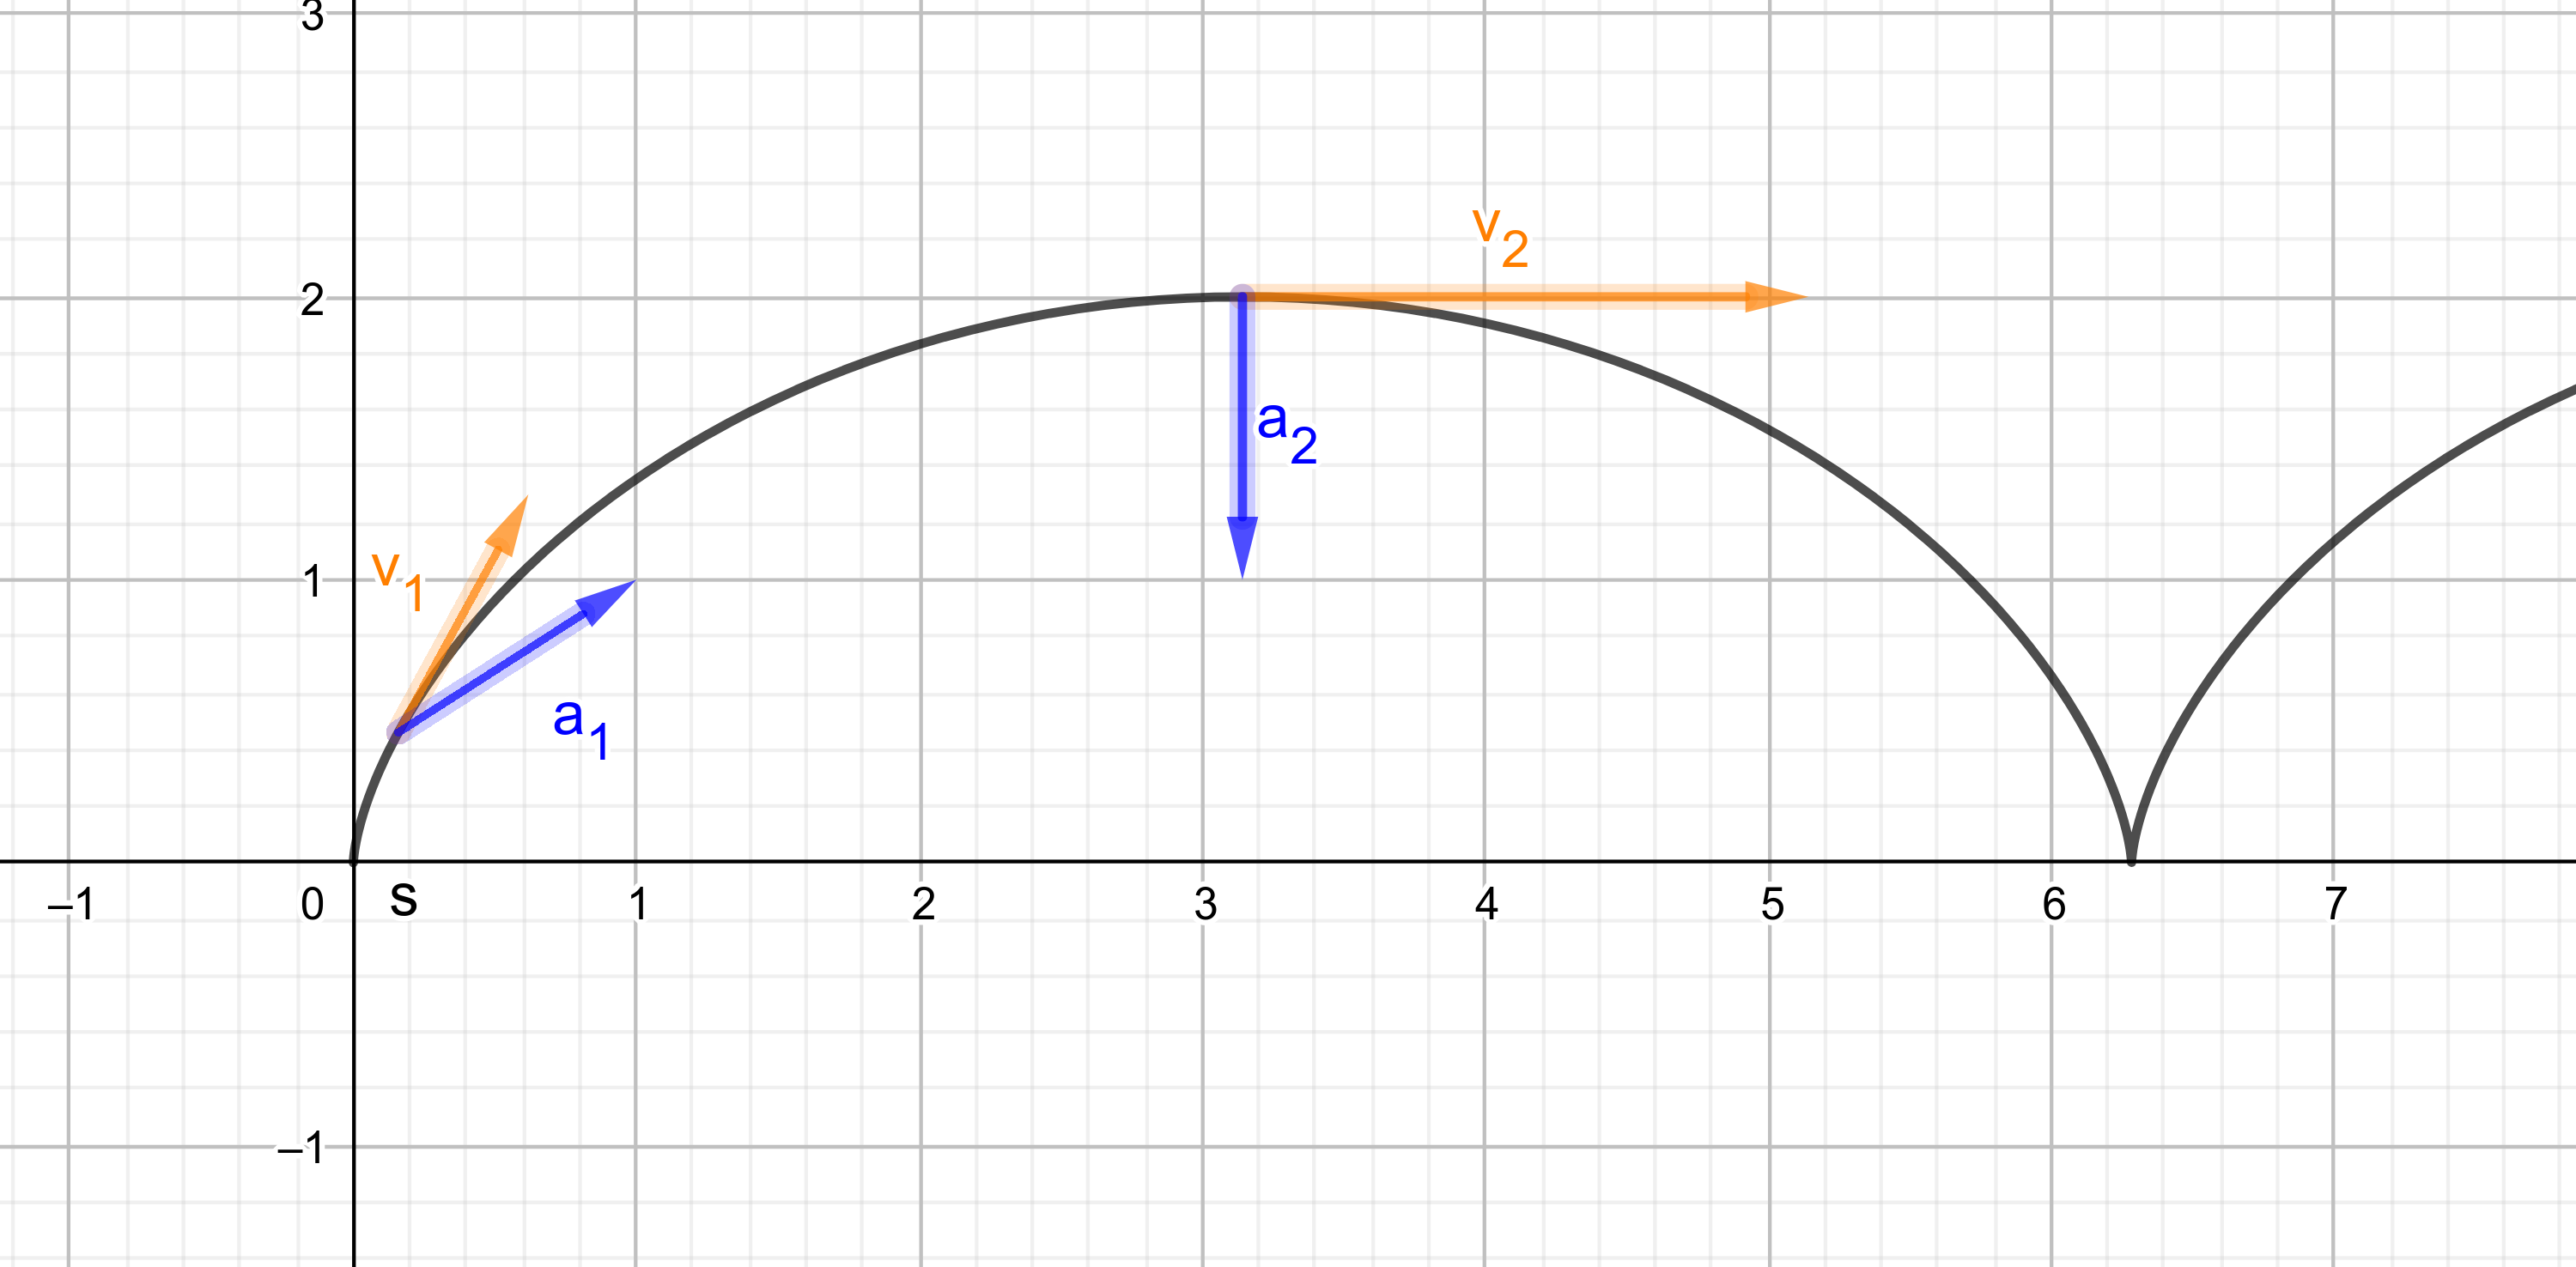
\includegraphics[scale=0.75]{./geogebra-export.png}\\
Diese Bahn entsteht, wenn man einen Punkt auf einem Kreis markiert, und anschließend den Kreis auf einer Geraden abrollt. Beispielsweise würde das Ventil eines Fahrradreifens näherungsweise diese Bahn beschreiben, wenn das Fahrrad fährt.

\end{document}
